\documentclass[aspectratio=169]{beamer}
\usepackage{booktabs}
\usepackage{pgfplots}
\pgfplotsset{compat=1.18}
\usepackage{tikz}
\usetikzlibrary{shapes.geometric,arrows.meta,positioning,fit,backgrounds,calc,decorations.pathreplacing,matrix}
\usepackage{xcolor}
\usepackage{colortbl}
\usepackage{multirow}
\usepackage{array}
\usepackage{amsmath}
\usepackage{listings}

\definecolor{TIRed}{RGB}{199,0,57}
\definecolor{TIBlue}{RGB}{0,71,133}
\definecolor{TIGold}{RGB}{255,180,0}
\definecolor{TIGreen}{RGB}{26,117,60}
\definecolor{TIGray}{RGB}{100,100,100}
\definecolor{LightGray}{RGB}{245,245,245}
\definecolor{AccentGreen}{RGB}{0,150,80}

\usetheme{Madrid}
\usecolortheme[named=TIBlue]{structure}
\setbeamercolor{title}{fg=white,bg=TIBlue}
\setbeamercolor{frametitle}{fg=white,bg=TIBlue}
\setbeamercolor{block title}{fg=white,bg=TIBlue}
\setbeamercolor{block title alerted}{fg=white,bg=TIRed}
\setbeamerfont{title}{size=\Large,series=\bfseries}
\setbeamerfont{frametitle}{size=\normalsize,series=\bfseries}
\setbeamertemplate{navigation symbols}{}
\setbeamertemplate{footline}[frame number]

\title{TI EdgeAI}
\subtitle{Hardware Products \& Model Zoo Fit Analysis}
\author{Edge AI Platform Evaluation}
\date{August 2026}
\institute{Texas Instruments}

\begin{document}

\begin{frame}\titlepage\end{frame}
\begin{frame}{Agenda}\tableofcontents\end{frame}

% ════════════════════════════════════════════════
\section{TI Edge AI Product Portfolio}
% ════════════════════════════════════════════════

\begin{frame}{TI Edge AI SoC Family Overview}
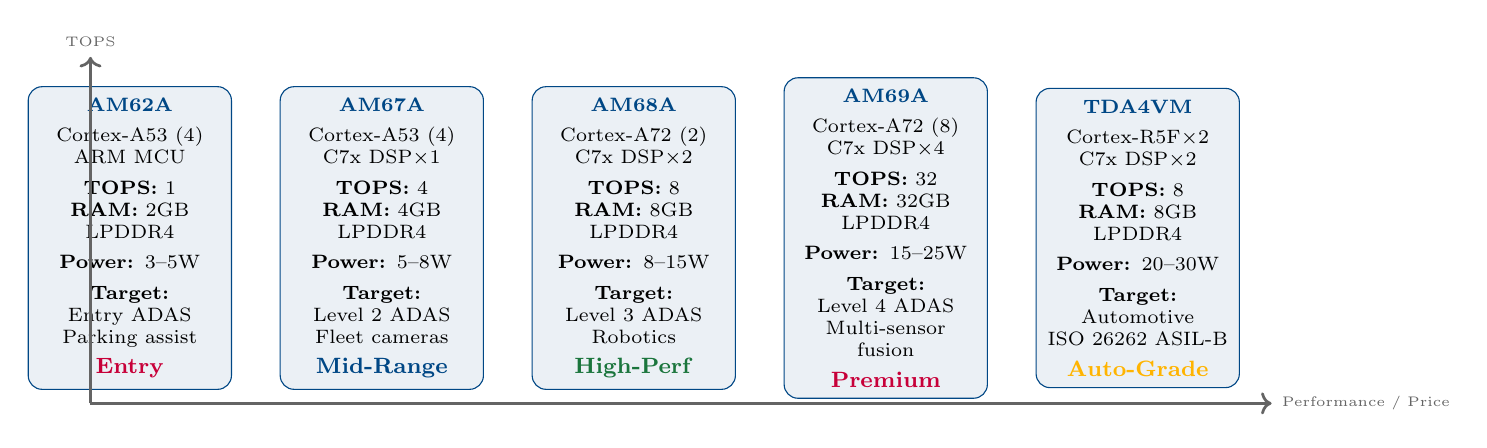
\begin{tikzpicture}[
  soc/.style={draw=TIBlue,fill=TIBlue!8,rounded corners=5pt,minimum width=2.5cm,
              minimum height=3.8cm,text width=2.3cm,align=center,font=\scriptsize,
              inner sep=4pt},
]
\node[soc] (am62a) at (0,0) {
  \textcolor{TIBlue}{\textbf{AM62A}}\\[3pt]
  Cortex-A53 (4)\\ARM MCU\\[3pt]
  \textbf{TOPS:} 1\\
  \textbf{RAM:} 2GB LPDDR4\\[3pt]
  \textbf{Power:} 3--5W\\[3pt]
  \textbf{Target:}\\Entry ADAS\\Parking assist\\[3pt]
  \footnotesize\textcolor{TIRed}{\textbf{Entry}}
};
\node[soc] (am67a) at (3.2,0) {
  \textcolor{TIBlue}{\textbf{AM67A}}\\[3pt]
  Cortex-A53 (4)\\C7x DSP$\times$1\\[3pt]
  \textbf{TOPS:} 4\\
  \textbf{RAM:} 4GB LPDDR4\\[3pt]
  \textbf{Power:} 5--8W\\[3pt]
  \textbf{Target:}\\Level 2 ADAS\\Fleet cameras\\[3pt]
  \footnotesize\textcolor{TIBlue}{\textbf{Mid-Range}}
};
\node[soc] (am68a) at (6.4,0) {
  \textcolor{TIBlue}{\textbf{AM68A}}\\[3pt]
  Cortex-A72 (2)\\C7x DSP$\times$2\\[3pt]
  \textbf{TOPS:} 8\\
  \textbf{RAM:} 8GB LPDDR4\\[3pt]
  \textbf{Power:} 8--15W\\[3pt]
  \textbf{Target:}\\Level 3 ADAS\\Robotics\\[3pt]
  \footnotesize\textcolor{TIGreen}{\textbf{High-Perf}}
};
\node[soc] (am69a) at (9.6,0) {
  \textcolor{TIBlue}{\textbf{AM69A}}\\[3pt]
  Cortex-A72 (8)\\C7x DSP$\times$4\\[3pt]
  \textbf{TOPS:} 32\\
  \textbf{RAM:} 32GB LPDDR4\\[3pt]
  \textbf{Power:} 15--25W\\[3pt]
  \textbf{Target:}\\Level 4 ADAS\\Multi-sensor fusion\\[3pt]
  \footnotesize\textcolor{TIRed}{\textbf{Premium}}
};
\node[soc] (tda4vm) at (12.8,0) {
  \textcolor{TIBlue}{\textbf{TDA4VM}}\\[3pt]
  Cortex-R5F$\times$2\\C7x DSP$\times$2\\[3pt]
  \textbf{TOPS:} 8\\
  \textbf{RAM:} 8GB LPDDR4\\[3pt]
  \textbf{Power:} 20--30W\\[3pt]
  \textbf{Target:}\\Automotive\\ISO 26262 ASIL-B\\[3pt]
  \footnotesize\textcolor{TIGold}{\textbf{Auto-Grade}}
};
\draw[->,line width=1pt,TIGray] (-0.5,-2.1) -- (14.5,-2.1)
  node[right,font=\tiny,text=TIGray]{Performance / Price};
\draw[->,line width=1pt,TIGray] (-0.5,-2.1) -- (-0.5,2.3)
  node[above,font=\tiny,text=TIGray]{TOPS};
\end{tikzpicture}
\end{frame}

\begin{frame}{TI Edge AI SoC Specifications Table}
\small
\begin{tabular}{lccccc}
\toprule
\textbf{Spec} & \textbf{AM62A} & \textbf{AM67A} & \textbf{AM68A} & \textbf{AM69A} & \textbf{TDA4VM}\\
\midrule
\textbf{NPU TOPS}    & 1.0      & 4.0      & 8.0       & 32.0      & 8.0\\
\textbf{CPU Cores}   & A53$\times$4 & A53$\times$4 & A72$\times$2 & A72$\times$8 & R5F$\times$2\\
\textbf{C7x DSP}     & 0        & 1        & 2         & 4         & 2\\
\textbf{Max RAM}     & 2 GB     & 4 GB     & 8 GB      & 32 GB     & 8 GB\\
\textbf{Power (TDP)} & 3--5 W   & 5--8 W   & 8--15 W   & 15--25 W  & 20--30 W\\
\textbf{Camera in}   & 2 CSI    & 4 CSI    & 6 CSI     & 8 CSI     & 8 CSI\\
\textbf{Video enc.}  & H.265    & H.265    & H.265 4K  & H.265 4K  & H.265 4K\\
\textbf{Safety}      & ---      & ---      & ---       & ---       & ASIL-B\\
\textbf{Process}     & 16 nm    & 16 nm    & 7 nm      & 7 nm      & 16 nm\\
\textbf{DRAM BW}     & 25.6 GB/s& 51.2 GB/s& 68 GB/s  & 204 GB/s  & 68 GB/s\\
\textbf{MSRP tier}   & Entry    & Mid      & High      & Premium   & Automotive\\
\midrule
\textbf{Primary use} & Parking  & Fleet cam& L3 ADAS   & L4 ADAS   & Auto OEM\\
\bottomrule
\end{tabular}
\end{frame}

\begin{frame}{TIDL NPU Architecture: MMA Core}
\begin{columns}
\column{0.52\textwidth}
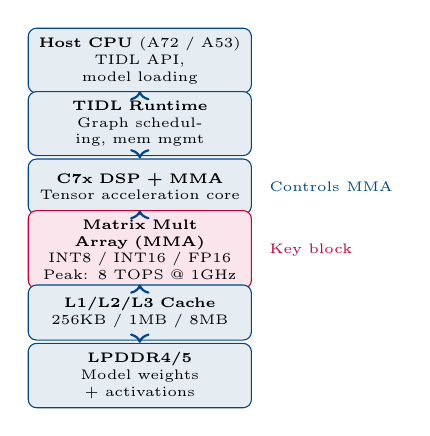
\begin{tikzpicture}[
  blk/.style={draw=TIBlue,fill=TIBlue!10,rounded corners=3pt,
              minimum height=0.7cm,text width=2.6cm,align=center,font=\tiny},
  sblk/.style={draw=TIRed,fill=TIRed!10,rounded corners=3pt,
               minimum height=0.7cm,text width=2.6cm,align=center,font=\tiny},
]
\node[blk] (cfg) at (0,4.2) {\textbf{Host CPU} (A72 / A53)\\TIDL API, model loading};
\node[blk] (tidlrt) at (0,3.4) {\textbf{TIDL Runtime}\\Graph scheduling, mem mgmt};
\node[blk] (c7x) at (0,2.6) {\textbf{C7x DSP + MMA}\\Tensor acceleration core};
\node[sblk] (mma) at (0,1.8) {\textbf{Matrix Mult Array (MMA)}\\INT8 / INT16 / FP16\\Peak: 8 TOPS @ 1GHz};
\node[blk] (cache) at (0,1.0) {\textbf{L1/L2/L3 Cache}\\256KB / 1MB / 8MB};
\node[blk] (ddr) at (0,0.2) {\textbf{LPDDR4/5}\\Model weights + activations};
\foreach \a/\b in {cfg/tidlrt,tidlrt/c7x,c7x/mma,mma/cache,cache/ddr}
  \draw[->,TIBlue,line width=0.8pt] (\a) -- (\b);
\node[right=0.1cm of mma,font=\tiny,text=TIRed] {Key block};
\node[right=0.1cm of c7x,font=\tiny,text=TIBlue] {Controls MMA};
\end{tikzpicture}
\column{0.45\textwidth}
\small
\begin{block}{MMA Key Facts}
\begin{itemize}
  \item \textbf{8-bit MAC array}: optimized INT8 matrix multiply
  \item \textbf{Per-layer precision}: mix INT8 + INT16 per layer
  \item \textbf{Data formats}: NCHW + NHWC both supported
  \item \textbf{Supported ops}: Conv2D, DepthwiseConv, Pooling, Concat, Eltwise, FC, Softmax
  \item \textbf{Layer fusion}: Conv+BN+ReLU in one pass
\end{itemize}
\end{block}
\begin{alertblock}{TIDL Whitelist}
\footnotesize Only operators on the \textbf{TIDL operator whitelist} run on NPU. Others fall back to C7x DSP or A72 CPU --- important for transformer models.
\end{alertblock}
\end{columns}
\end{frame}

% ════════════════════════════════════════════════
\section{TIDL Software Stack}
% ════════════════════════════════════════════════

\begin{frame}{TIDL Software Stack: End-to-End Flow}
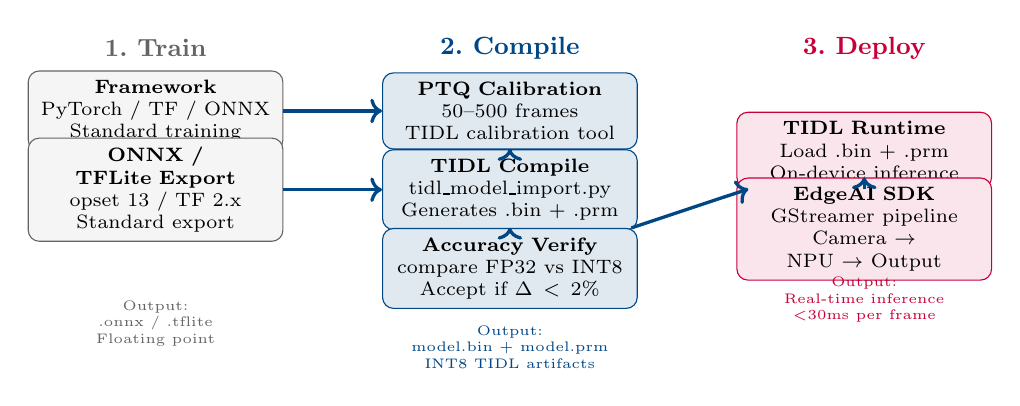
\begin{tikzpicture}[
  box/.style={rounded corners=4pt,minimum height=0.85cm,
              text width=3.0cm,align=center,font=\scriptsize},
  arr/.style={->,line width=1.2pt,TIBlue},
]
\node[draw=TIGray,fill=LightGray,box] (fw) at (0,3.0)
  {\textbf{Framework}\\PyTorch / TF / ONNX\\Standard training};
\node[draw=TIGray,fill=LightGray,box] (exp) at (0,2.0)
  {\textbf{ONNX / TFLite Export}\\opset 13 / TF 2.x\\Standard export};
\node[draw=TIBlue,fill=TIBlue!12,box] (calib) at (4.5,3.0)
  {\textbf{PTQ Calibration}\\50--500 frames\\TIDL calibration tool};
\node[draw=TIBlue,fill=TIBlue!12,box] (compile) at (4.5,2.0)
  {\textbf{TIDL Compile}\\tidl\_model\_import.py\\Generates .bin + .prm};
\node[draw=TIBlue,fill=TIBlue!12,box] (opt) at (4.5,1.0)
  {\textbf{Accuracy Verify}\\compare FP32 vs INT8\\Accept if $\Delta < 2\%$};
\node[draw=TIRed,fill=TIRed!10,box] (rt) at (9.0,2.5)
  {\textbf{TIDL Runtime}\\Load .bin + .prm\\On-device inference};
\node[draw=TIRed,fill=TIRed!10,box] (sdk) at (9.0,1.5)
  {\textbf{EdgeAI SDK}\\GStreamer pipeline\\Camera $\to$ NPU $\to$ Output};
\draw[arr] (fw) -- (calib);
\draw[arr] (exp) -- (compile);
\draw[arr] (compile) -- (opt);
\draw[arr] (calib) -- (compile);
\draw[arr] (opt) -- (rt);
\draw[arr] (rt) -- (sdk);
\node[font=\small\bfseries,text=TIGray] at (0,3.8) {1.\ Train};
\node[font=\small\bfseries,text=TIBlue] at (4.5,3.8) {2.\ Compile};
\node[font=\small\bfseries,text=TIRed] at (9.0,3.8) {3.\ Deploy};
\node[font=\tiny,text=TIGray,align=center] at (0,0.3)
  {Output:\\.onnx / .tflite\\Floating point};
\node[font=\tiny,text=TIBlue,align=center] at (4.5,0.0)
  {Output:\\model.bin + model.prm\\INT8 TIDL artifacts};
\node[font=\tiny,text=TIRed,align=center] at (9.0,0.6)
  {Output:\\Real-time inference\\$<$30ms per frame};
\end{tikzpicture}
\end{frame}

\begin{frame}{edgeai-modelzoo Repository Structure}
\begin{columns}
\column{0.48\textwidth}
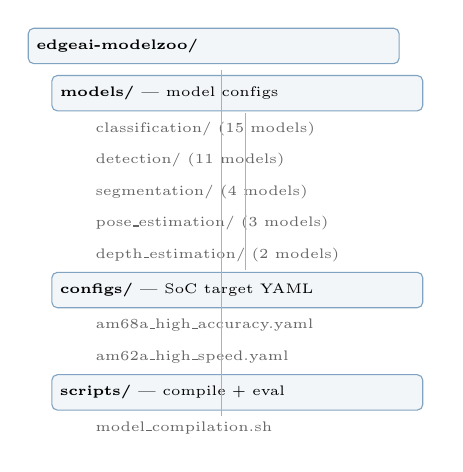
\begin{tikzpicture}[
  dir/.style={draw=TIBlue!50,fill=TIBlue!5,rounded corners=2pt,
              font=\tiny,minimum height=0.45cm,text width=4.5cm,
              align=left,inner sep=3pt},
  file/.style={font=\tiny,text=TIGray,minimum height=0.4cm,
               text width=4.2cm,align=left,inner sep=3pt},
]
\node[dir] at (0,5.0) {\textbf{edgeai-modelzoo/}};
\node[dir] at (0.3,4.4) {\textbf{models/}  --- model configs};
\node[file] at (0.6,3.95) {classification/ (15 models)};
\node[file] at (0.6,3.55) {detection/ (11 models)};
\node[file] at (0.6,3.15) {segmentation/ (4 models)};
\node[file] at (0.6,2.75) {pose\_estimation/ (3 models)};
\node[file] at (0.6,2.35) {depth\_estimation/ (2 models)};
\node[dir] at (0.3,1.9) {\textbf{configs/} --- SoC target YAML};
\node[file] at (0.6,1.45) {am68a\_high\_accuracy.yaml};
\node[file] at (0.6,1.05) {am62a\_high\_speed.yaml};
\node[dir] at (0.3,0.6) {\textbf{scripts/} --- compile + eval};
\node[file] at (0.6,0.15) {model\_compilation.sh};
\draw[-,TIBlue!40] (0.1,4.7) -- (0.1,0.3);
\draw[-,TIBlue!40] (0.4,4.15) -- (0.4,2.15);
\end{tikzpicture}
\column{0.48\textwidth}
\small
\begin{block}{Model Config Format}
\footnotesize
\begin{verbatim}
model_id: yolox-s-lite
input_size: [1,3,640,640]
task_type: object_detection
target_device: AM68A
tidl_calibration_frames: 100
accuracy_threshold: 36.0  # mAP
source_model: yolox_s.onnx
\end{verbatim}
\end{block}
\begin{block}{Per-SoC YAML}
\footnotesize
\begin{verbatim}
soc: AM68A
tidl_tools_path: /opt/tidl_tools
num_bits: 8
max_mem_banks: 32
deny_list_layers: []
\end{verbatim}
\end{block}
\end{columns}
\end{frame}

% ════════════════════════════════════════════════
\section{Model Zoo: Classification Models}
% ════════════════════════════════════════════════

\begin{frame}{Classification Models --- Hardware Fit Matrix}
\small
\begin{tabular}{lcccccp{2.5cm}}
\toprule
\textbf{Model} & \textbf{Top-1} & \textbf{Size} & \textbf{AM62A} & \textbf{AM67A} & \textbf{AM68A+} & \textbf{Why fits}\\
\midrule
mobilenet\_v2\_lite      & 72.3\% & 3.4M  & \textcolor{AccentGreen}{\checkmark\checkmark} & \checkmark & \checkmark & Depthwise conv, TIDL-friendly, fits 1 TOPS\\
mobilenet\_v3\_small\_lite & 67.2\% & 2.5M & \textcolor{AccentGreen}{\checkmark\checkmark} & \checkmark & \checkmark & SE layers map to TIDL Eltwise ops\\
mobilenet\_v3\_large\_lite & 74.8\% & 5.4M & \checkmark & \textcolor{AccentGreen}{\checkmark\checkmark} & \checkmark & Needs 4 TOPS for real-time 30FPS\\
regnet\_x\_400mf\_lite   & 74.1\% & 5.2M  & \checkmark & \textcolor{AccentGreen}{\checkmark\checkmark} & \checkmark & Group conv TIDL-supported\\
regnet\_x\_800mf\_lite   & 75.2\% & 7.3M  & $\circ$ & \textcolor{AccentGreen}{\checkmark\checkmark} & \checkmark & $\sim$2 TOPS required\\
efficientnet\_b0\_lite   & 76.3\% & 5.3M  & $\circ$ & \checkmark & \textcolor{AccentGreen}{\checkmark\checkmark} & SE blocks, BN folding needed\\
resnet18\_lite           & 71.5\% & 11.7M & $\circ$ & \checkmark & \textcolor{AccentGreen}{\checkmark\checkmark} & Residual add = Eltwise on TIDL\\
vgg16\_lite              & 73.8\% & 138M  & $\times$ & $\circ$ & \textcolor{AccentGreen}{\checkmark\checkmark} & Large weights, needs 8 GB LPDDR4\\
fastvit\_s12             & 79.3\% & 7.8M  & $\times$ & $\circ$ & \textcolor{AccentGreen}{\checkmark\checkmark} & Partial CPU fallback for MixToken\\
swin\_tiny               & 81.2\% & 28M   & $\times$ & $\times$ & \textcolor{AccentGreen}{\checkmark\checkmark} & W-MSA partial NPU; needs 8 TOPS\\
\midrule
\multicolumn{7}{l}{\footnotesize \textcolor{AccentGreen}{\checkmark\checkmark} = optimal fit \quad \checkmark = supported \quad $\circ$ = possible \quad $\times$ = not recommended}
\end{tabular}
\end{frame}

\begin{frame}{Classification Accuracy by Target SoC}
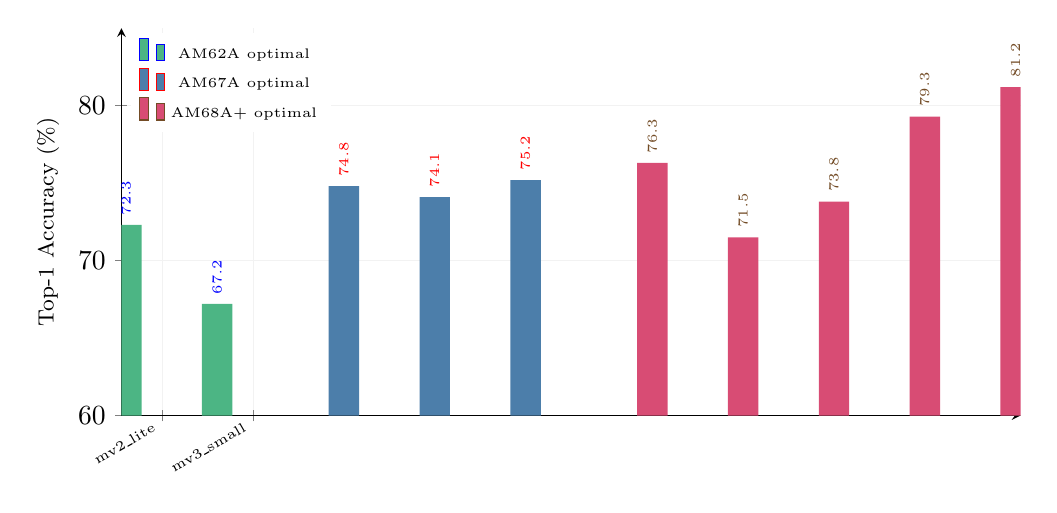
\begin{tikzpicture}
\begin{axis}[
  ybar,
  width=13cm, height=6.5cm,
  bar width=11pt,
  ylabel={\footnotesize Top-1 Accuracy (\%)},
  xtick=data,
  xticklabels={mv2\_lite,mv3\_small,mv3\_large,regx400,regx800,effb0,res18,vgg16,fastvit,swin\_t},
  xticklabel style={font=\tiny,rotate=30,anchor=east},
  ymin=60,ymax=85,
  grid=major,grid style={gray!10},
  axis lines=left,
  legend style={font=\tiny,at={(0.01,0.99)},anchor=north west,draw=none},
  nodes near coords,
  nodes near coords style={font=\tiny,rotate=90,anchor=west},
  every node near coord/.append style={/pgf/number format/.cd,fixed,precision=1},
  enlarge x limits=0.05,
]
\addplot+[fill=AccentGreen!70,draw=none] coordinates {(0,72.3)(1,67.2)};
\addlegendentry{AM62A optimal}
\addplot+[fill=TIBlue!70,draw=none] coordinates {(2,74.8)(3,74.1)(4,75.2)};
\addlegendentry{AM67A optimal}
\addplot+[fill=TIRed!70,draw=none] coordinates {(5,76.3)(6,71.5)(7,73.8)(8,79.3)(9,81.2)};
\addlegendentry{AM68A+ optimal}
\end{axis}
\end{tikzpicture}
\end{frame}

% ════════════════════════════════════════════════
\section{Model Zoo: Detection Models}
% ════════════════════════════════════════════════

\begin{frame}{Detection Models --- SoC Fit \& Latency}
\small
\begin{tabular}{lccccl}
\toprule
\textbf{Model} & \textbf{mAP} & \textbf{Input} & \textbf{Optimal SoC} & \textbf{Latency} & \textbf{Why fits}\\
\midrule
yolox\_pico\_lite & 20.1\% & 320$\times$320 & AM62A  & $\sim$8ms  & Tiny: 0.9M params, 1 TOPS sufficient\\
yolox\_nano\_lite & 22.4\% & 416$\times$416 & AM62A  & $\sim$12ms & Single head, no FPN, low mem BW\\
yolox\_tiny\_lite & 29.2\% & 416$\times$416 & AM67A  & $\sim$18ms & FPN starts here; needs 4 TOPS\\
yolox\_s\_lite    & 38.4\% & 640$\times$640 & AM67A  & $\sim$28ms & Standard FPN + PAN, 8.9M params\\
yolox\_m\_lite    & 44.2\% & 640$\times$640 & AM68A  & $\sim$45ms & 25M params; needs 8 TOPS\\
yolox\_l\_lite    & 49.0\% & 640$\times$640 & AM68A  & $\sim$65ms & 54M params; 8 GB LPDDR4 needed\\
yolov7\_l\_lite   & 51.0\% & 640$\times$640 & AM68A  & $\sim$55ms & Multi-branch; E-ELAN on TIDL\\
rtmdet\_m\_lite   & 56.0\% & 640$\times$640 & AM69A  & $\sim$40ms & CSPNext backbone; 4 DSPs optimal\\
rtmdet\_l\_lite   & 60.0\% & 640$\times$640 & AM69A  & $\sim$60ms & Largest det model; 32 TOPS shines\\
peoplenet\_lite   & 85.0\% & 960$\times$544 & TDA4VM & $\sim$20ms & Automotive NvDet variant, ASIL-B\\
\midrule
\multicolumn{6}{l}{\footnotesize All mAP on COCO val2017 \quad Latency measured on target SoC NPU}
\end{tabular}
\end{frame}

\begin{frame}{Detection mAP vs.\ Latency: Efficiency Frontier}
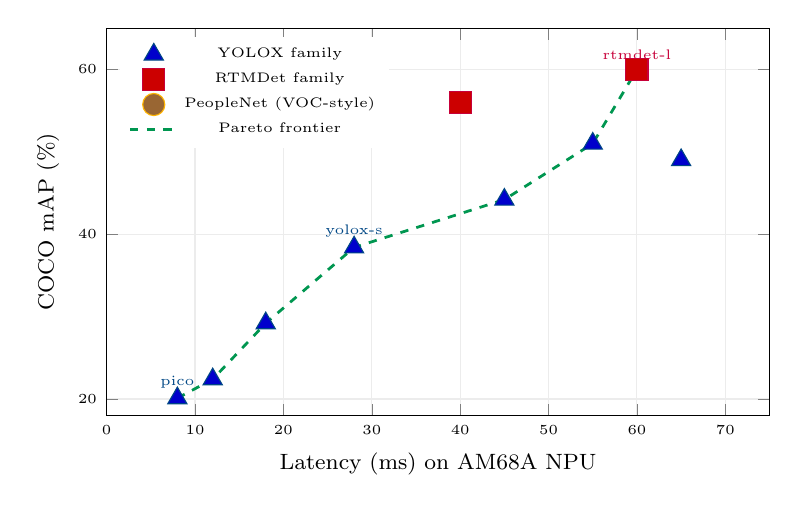
\begin{tikzpicture}
\begin{axis}[
  width=10cm, height=6.5cm,
  xlabel={\footnotesize Latency (ms) on AM68A NPU},
  ylabel={\footnotesize COCO mAP (\%)},
  xmin=0, xmax=75,
  ymin=18, ymax=65,
  grid=major, grid style={gray!15},
  legend style={font=\tiny,at={(0.02,0.98)},anchor=north west,draw=none},
  xlabel style={font=\tiny},
  ylabel style={font=\tiny},
  xticklabel style={font=\tiny},
  yticklabel style={font=\tiny},
]
\addplot+[only marks,mark=triangle*,mark size=4pt,color=TIBlue]
  coordinates {(8,20.1)(12,22.4)(18,29.2)(28,38.4)(45,44.2)(65,49.0)(55,51.0)};
\addlegendentry{YOLOX family}
\addplot+[only marks,mark=square*,mark size=4pt,color=TIRed]
  coordinates {(40,56.0)(60,60.0)};
\addlegendentry{RTMDet family}
\addplot+[only marks,mark=*,mark size=4pt,color=TIGold]
  coordinates {(20,85.0)};
\addlegendentry{PeopleNet (VOC-style)}
\addplot+[no marks,dashed,color=AccentGreen,line width=1pt]
  coordinates {(8,20.1)(12,22.4)(18,29.2)(28,38.4)(45,44.2)(55,51.0)(60,60.0)};
\addlegendentry{Pareto frontier}
% Annotations
\node[font=\tiny,text=TIBlue,anchor=south] at (axis cs:8,20.1) {pico};
\node[font=\tiny,text=TIBlue,anchor=south] at (axis cs:28,38.4) {yolox-s};
\node[font=\tiny,text=TIRed,anchor=south] at (axis cs:60,60.0) {rtmdet-l};
\node[font=\tiny,text=TIGold,anchor=west] at (axis cs:21,85.0) {peoplenet};
\end{axis}
\end{tikzpicture}
\end{frame}

\begin{frame}{YOLOX Family: Architecture Fit to MMA}
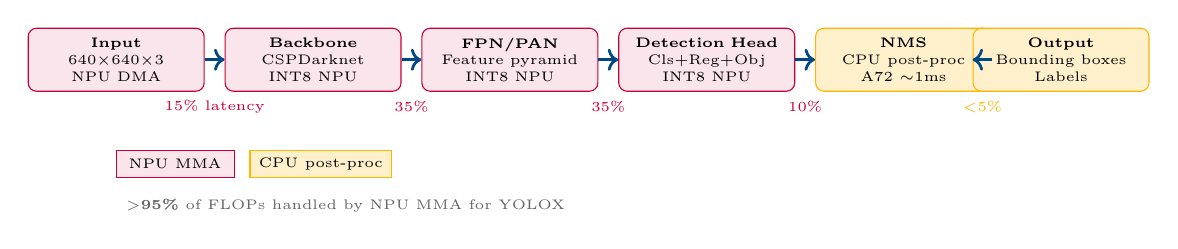
\begin{tikzpicture}[
  npu/.style={draw=TIRed,fill=TIRed!10,rounded corners=3pt,
              minimum height=0.8cm,text width=2.0cm,align=center,font=\tiny},
  cpu/.style={draw=TIGold,fill=TIGold!20,rounded corners=3pt,
              minimum height=0.8cm,text width=2.0cm,align=center,font=\tiny},
]
\node[npu] (in)   at (0,2)   {\textbf{Input}\\640$\times$640$\times$3\\NPU DMA};
\node[npu] (b1)   at (2.5,2) {\textbf{Backbone}\\CSPDarknet\\INT8 NPU};
\node[npu] (fpn)  at (5.0,2) {\textbf{FPN/PAN}\\Feature pyramid\\INT8 NPU};
\node[npu] (head) at (7.5,2) {\textbf{Detection Head}\\Cls+Reg+Obj\\INT8 NPU};
\node[cpu] (nms)  at (10,2)  {\textbf{NMS}\\CPU post-proc\\A72 $\sim$1ms};
\node[cpu] (out)  at (12,2)  {\textbf{Output}\\Bounding boxes\\Labels};
\draw[->,TIBlue,line width=1pt] (in) -- (b1);
\draw[->,TIBlue,line width=1pt] (b1) -- (fpn);
\draw[->,TIBlue,line width=1pt] (fpn) -- (head);
\draw[->,TIBlue,line width=1pt] (head) -- (nms);
\draw[->,TIBlue,line width=1pt] (nms) -- (out);
\node[font=\tiny,text=TIRed] at (1.25,1.4) {15\% latency};
\node[font=\tiny,text=TIRed] at (3.75,1.4) {35\%};
\node[font=\tiny,text=TIRed] at (6.25,1.4) {35\%};
\node[font=\tiny,text=TIRed] at (8.75,1.4) {10\%};
\node[font=\tiny,text=TIGold] at (11.0,1.4) {$<$5\%};
\draw[fill=TIRed!10,draw=TIRed] (0,0.5) rectangle (1.5,0.85)
  node[midway,font=\tiny]{NPU MMA};
\draw[fill=TIGold!20,draw=TIGold] (1.7,0.5) rectangle (3.5,0.85)
  node[midway,font=\tiny]{CPU post-proc};
\node[font=\tiny,text=TIGray,anchor=west] at (0,0.15)
  {\textbf{$>$95\%} of FLOPs handled by NPU MMA for YOLOX};
\end{tikzpicture}
\end{frame}

% ════════════════════════════════════════════════
\section{Model Zoo: Segmentation, Pose \& Depth}
% ════════════════════════════════════════════════

\begin{frame}{Segmentation, Pose, Depth --- Hardware Requirements}
\begin{columns}
\column{0.55\textwidth}
\small
\begin{tabular}{lccl}
\toprule
\textbf{Model} & \textbf{Metric} & \textbf{Target} & \textbf{Key constraint}\\
\midrule
\multicolumn{4}{l}{\textit{Segmentation}}\\
deeplabv3plus\_lite   & 65.3\% mIoU & AM68A & ASPP: 6 dilated convs\\
fpn\_regnetx800\_lite & 55.2\% mIoU & AM67A & Light FPN only\\
unet\_jseg\_lite      & 67.0\% mIoU & AM68A & Skip connections\\
bisenetv2\_lite       & 61.0\% mIoU & AM67A & Dual-path supported\\
\midrule
\multicolumn{4}{l}{\textit{Pose Estimation}}\\
yoloxpose\_s\_lite & AP 61.2\% & AM68A & Heatmap + OKS loss\\
yoloxpose\_m\_lite & AP 66.8\% & AM68A & 17 keypoints COCO\\
yoloxpose\_l\_lite & AP 70.1\% & AM69A & Large: 4 DSPs optimal\\
\midrule
\multicolumn{4}{l}{\textit{Depth Estimation}}\\
fastdepth\_lite    & err 15.8\% & AM67A & BN fusion critical\\
midas\_small\_lite & err 13.2\% & AM68A & Mix-decoder ops\\
\bottomrule
\end{tabular}
\column{0.42\textwidth}
\footnotesize
\begin{block}{Why Segmentation Needs AM68A}
\begin{itemize}
  \item ASPP requires multiple parallel conv branches --- needs 8 TOPS for real-time
  \item High-res feature maps (512$\times$512) exceed LPDDR4 BW on AM62A
  \item TIDL supports dilated conv natively
\end{itemize}
\end{block}
\begin{block}{Depth Estimation Trick}
MonoDepth models use BN fusion during TIDL compile to halve activation memory --- critical for fitting 512$\times$512 inputs on AM67A's 4 GB.
\end{block}
\end{columns}
\end{frame}

% ════════════════════════════════════════════════
\section{Why Model Zoo Models Fit TI Hardware}
% ════════════════════════════════════════════════

\begin{frame}{Model Zoo Design Principles for TIDL}
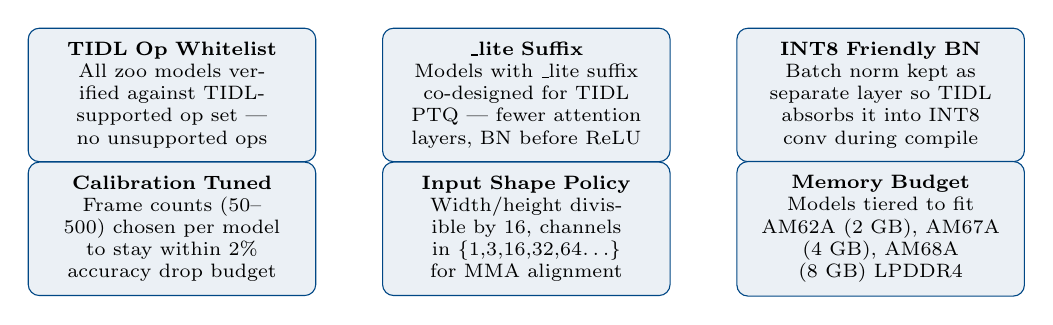
\begin{tikzpicture}[
  principle/.style={draw=TIBlue,fill=TIBlue!8,rounded corners=4pt,
                    minimum height=1.4cm,text width=3.3cm,align=center,
                    font=\scriptsize,inner sep=5pt},
]
\node[principle] at (0,2.5) {\textbf{TIDL Op Whitelist}\\All zoo models verified against TIDL-supported op set --- no unsupported ops};
\node[principle] at (4.5,2.5) {\textbf{\_lite Suffix}\\Models with \_lite suffix co-designed for TIDL PTQ --- fewer attention layers, BN before ReLU};
\node[principle] at (9.0,2.5) {\textbf{INT8 Friendly BN}\\Batch norm kept as separate layer so TIDL absorbs it into INT8 conv during compile};
\node[principle] at (0,0.8) {\textbf{Calibration Tuned}\\Frame counts (50--500) chosen per model to stay within 2\% accuracy drop budget};
\node[principle] at (4.5,0.8) {\textbf{Input Shape Policy}\\Width/height divisible by 16, channels in $\{$1,3,16,32,64$\ldots\}$ for MMA alignment};
\node[principle] at (9.0,0.8) {\textbf{Memory Budget}\\Models tiered to fit AM62A (2 GB), AM67A (4 GB), AM68A (8 GB) LPDDR4};
\end{tikzpicture}
\end{frame}

\begin{frame}{TIDL Operator Support --- Key Model Families}
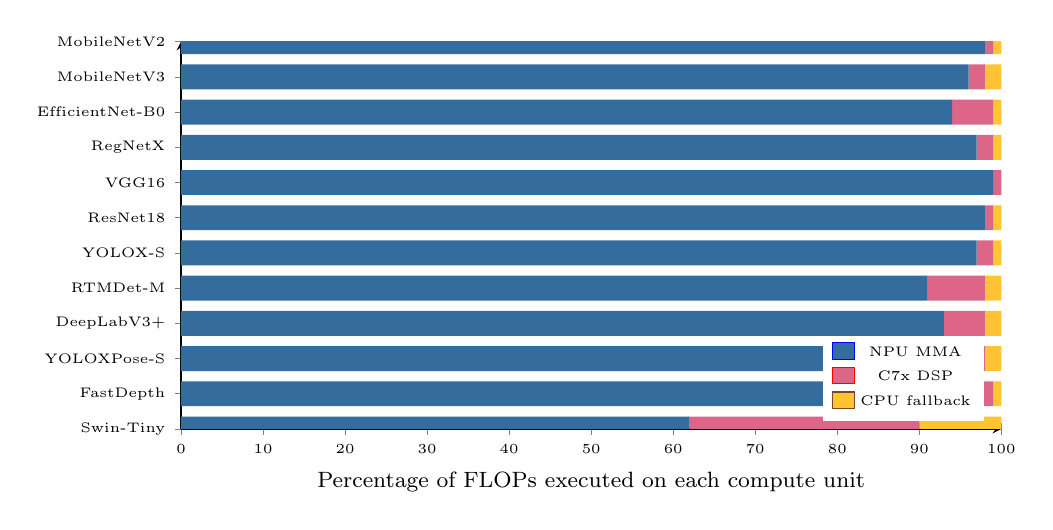
\begin{tikzpicture}
\begin{axis}[
  xbar stacked,
  width=12cm, height=6.5cm,
  bar width=9pt,
  xlabel={\footnotesize Percentage of FLOPs executed on each compute unit},
  ytick=data,
  yticklabels={
    MobileNetV2,MobileNetV3,EfficientNet-B0,RegNetX,VGG16,ResNet18,
    YOLOX-S,RTMDet-M,DeepLabV3+,YOLOXPose-S,FastDepth,Swin-Tiny
  },
  yticklabel style={font=\tiny},
  xticklabel style={font=\tiny},
  xlabel style={font=\tiny},
  legend style={font=\tiny,at={(0.98,0.02)},anchor=south east,draw=none},
  xmin=0,xmax=100,
  tick align=inside,axis lines=left,
]
\addplot+[xbar,fill=TIBlue!80,draw=none] coordinates {
  (98,11)(96,10)(94,9)(97,8)(99,7)(98,6)
  (97,5)(91,4)(93,3)(95,2)(97,1)(62,0)};
\addplot+[xbar,fill=TIRed!60,draw=none] coordinates {
  (1,11)(2,10)(5,9)(2,8)(1,7)(1,6)
  (2,5)(7,4)(5,3)(3,2)(2,1)(28,0)};
\addplot+[xbar,fill=TIGold!80,draw=none] coordinates {
  (1,11)(2,10)(1,9)(1,8)(0,7)(1,6)
  (1,5)(2,4)(2,3)(2,2)(1,1)(10,0)};
\legend{NPU MMA,C7x DSP,CPU fallback}
\end{axis}
\end{tikzpicture}
\vspace{2pt}
\footnotesize\textcolor{TIGray}{Swin-Tiny W-MSA (window attention) partially falls back to CPU --- all CNN models $>$90\% on NPU.}
\end{frame}

\begin{frame}{Memory Fit: Weights + Activations per SoC}
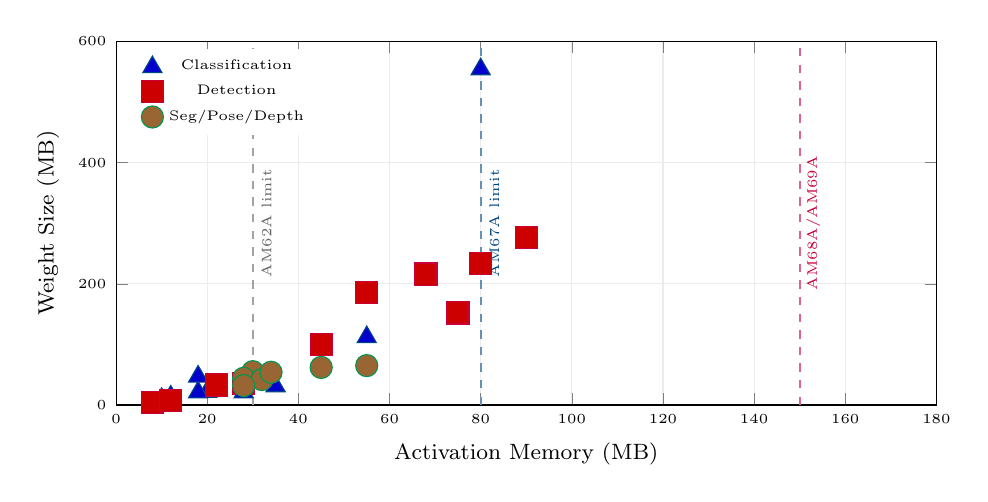
\begin{tikzpicture}
\begin{axis}[
  width=12cm, height=6.2cm,
  xlabel={\footnotesize Activation Memory (MB)},
  ylabel={\footnotesize Weight Size (MB)},
  xmin=0,xmax=180,
  ymin=0,ymax=600,
  grid=major,grid style={gray!15},
  legend style={font=\tiny,at={(0.02,0.98)},anchor=north west,draw=none},
  xlabel style={font=\tiny},
  ylabel style={font=\tiny},
  xticklabel style={font=\tiny},
  yticklabel style={font=\tiny},
]
\draw[dashed,TIGray!60,line width=0.8pt] (axis cs:30,0) -- (axis cs:30,600);
\node[font=\tiny,text=TIGray,rotate=90] at (axis cs:33,300) {AM62A limit};
\draw[dashed,TIBlue!60,line width=0.8pt] (axis cs:80,0) -- (axis cs:80,600);
\node[font=\tiny,text=TIBlue,rotate=90] at (axis cs:83,300) {AM67A limit};
\draw[dashed,TIRed!60,line width=0.8pt] (axis cs:150,0) -- (axis cs:150,600);
\node[font=\tiny,text=TIRed,rotate=90] at (axis cs:153,300) {AM68A/AM69A};
\addplot+[only marks,mark=triangle*,mark size=4pt,color=TIBlue]
  coordinates {(12,14)(10,10)(20,22)(18,21)(22,29)(28,21)(18,47)(80,554)(35,31)(55,112)};
\addlegendentry{Classification}
\addplot+[only marks,mark=square*,mark size=4pt,color=TIRed]
  coordinates {(8,3.6)(12,7.2)(22,33)(28,36)(45,100)(68,216)(55,186)(75,152)(80,234)(90,276)};
\addlegendentry{Detection}
\addplot+[only marks,mark=*,mark size=4pt,color=AccentGreen]
  coordinates {(45,62)(30,55)(55,65)(28,44)(32,42)(34,54)(28,32)};
\addlegendentry{Seg/Pose/Depth}
\end{axis}
\end{tikzpicture}
\end{frame}

% ════════════════════════════════════════════════
\section{Performance Benchmarks}
% ════════════════════════════════════════════════

\begin{frame}{Inference Latency on AM68A --- All 29 Vision Models}
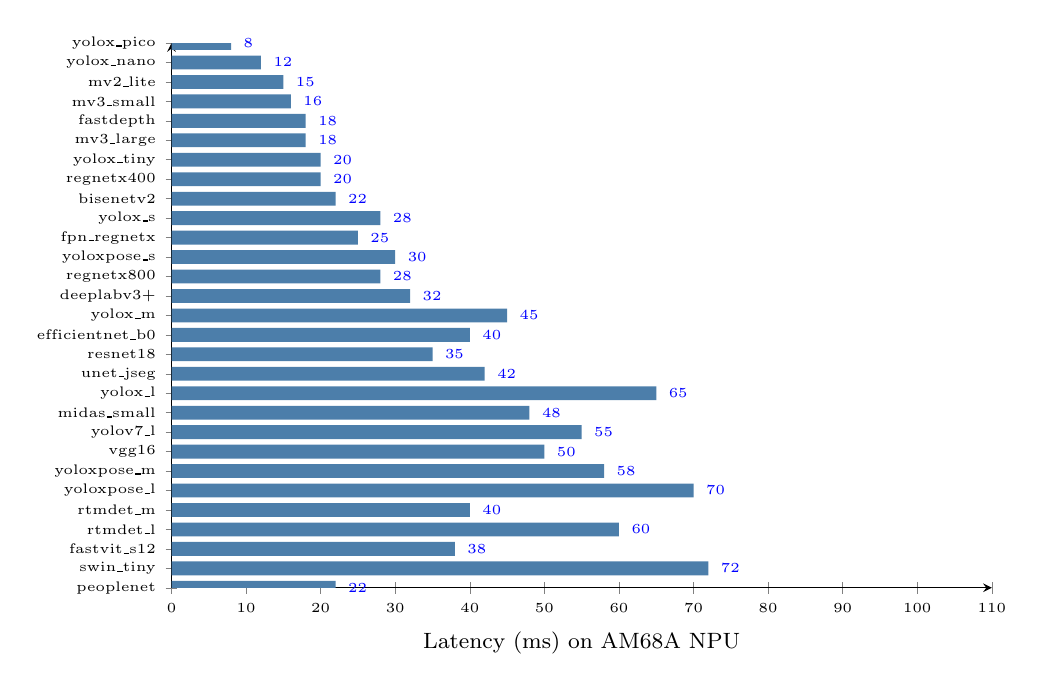
\begin{tikzpicture}
\begin{axis}[
  xbar,
  width=12cm, height=8.5cm,
  bar width=5pt,
  xlabel={\footnotesize Latency (ms) on AM68A NPU},
  ytick=data,
  yticklabels={
    yolox\_pico,yolox\_nano,mv2\_lite,mv3\_small,fastdepth,mv3\_large,
    yolox\_tiny,regnetx400,bisenetv2,yolox\_s,fpn\_regnetx,yoloxpose\_s,
    regnetx800,deeplabv3+,yolox\_m,efficientnet\_b0,resnet18,unet\_jseg,
    yolox\_l,midas\_small,yolov7\_l,vgg16,yoloxpose\_m,yoloxpose\_l,
    rtmdet\_m,rtmdet\_l,fastvit\_s12,swin\_tiny,peoplenet
  },
  yticklabel style={font=\tiny},
  xticklabel style={font=\tiny},
  xmin=0,xmax=110,
  tick align=inside,axis lines=left,
  nodes near coords,
  nodes near coords style={font=\tiny,xshift=1pt},
]
\addplot+[xbar,fill=TIBlue!70,draw=none] coordinates {
  (8,28)(12,27)(15,26)(16,25)(18,24)(18,23)
  (20,22)(20,21)(22,20)(28,19)(25,18)(30,17)
  (28,16)(32,15)(45,14)(40,13)(35,12)(42,11)
  (65,10)(48,9)(55,8)(50,7)(58,6)(70,5)
  (40,4)(60,3)(38,2)(72,1)(22,0)
};
\end{axis}
\end{tikzpicture}
\end{frame}

\begin{frame}{FPS Comparison: AM62A vs AM67A vs AM68A}
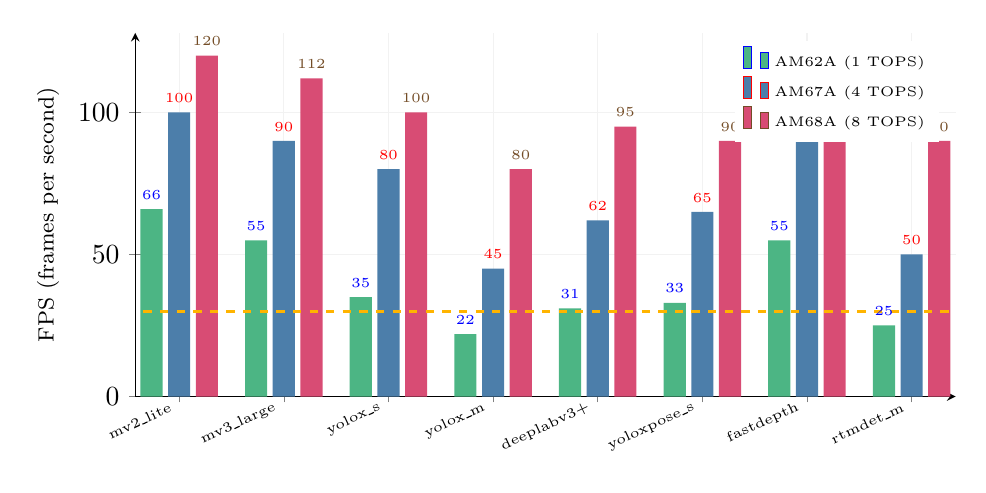
\begin{tikzpicture}
\begin{axis}[
  ybar,
  width=12cm, height=6.2cm,
  bar width=8pt,
  ylabel={\footnotesize FPS (frames per second)},
  xtick=data,
  xticklabels={mv2\_lite,mv3\_large,yolox\_s,yolox\_m,deeplabv3+,yoloxpose\_s,fastdepth,rtmdet\_m},
  xticklabel style={font=\tiny,rotate=25,anchor=east},
  ymin=0,ymax=128,
  grid=major,grid style={gray!10},
  axis lines=left,
  legend style={font=\tiny,at={(0.98,0.98)},anchor=north east,draw=none},
  nodes near coords,nodes near coords style={font=\tiny},
  enlarge x limits=0.06,
]
\addplot+[fill=AccentGreen!70,draw=none]
  coordinates {(0,66)(1,55)(2,35)(3,22)(4,31)(5,33)(6,55)(7,25)};
\addlegendentry{AM62A (1 TOPS)}
\addplot+[fill=TIBlue!70,draw=none]
  coordinates {(0,100)(1,90)(2,80)(3,45)(4,62)(5,65)(6,95)(7,50)};
\addlegendentry{AM67A (4 TOPS)}
\addplot+[fill=TIRed!70,draw=none]
  coordinates {(0,120)(1,112)(2,100)(3,80)(4,95)(5,90)(6,115)(7,90)};
\addlegendentry{AM68A (8 TOPS)}
\draw[dashed,TIGold,line width=1.2pt] (axis cs:-0.5,30) -- (axis cs:7.5,30)
  node[right,font=\tiny,text=TIGold]{30 FPS target};
\end{axis}
\end{tikzpicture}
\end{frame}

\begin{frame}{Accuracy Retention: FP32 $\rightarrow$ INT8 PTQ}
\begin{columns}
\column{0.58\textwidth}
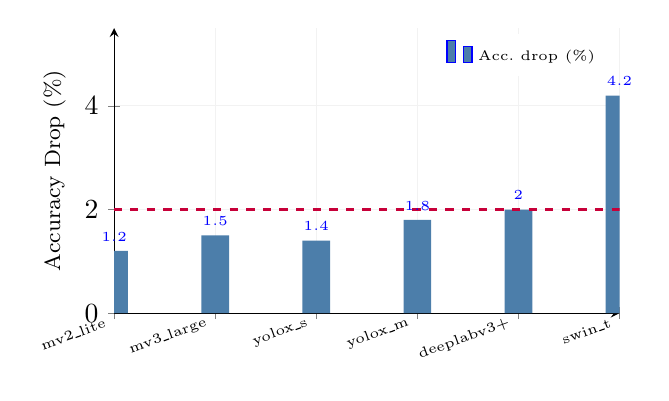
\begin{tikzpicture}
\begin{axis}[
  ybar,
  width=8cm, height=5.2cm,
  bar width=10pt,
  ylabel={\footnotesize Accuracy Drop (\%)},
  xtick=data,
  xticklabels={mv2\_lite,mv3\_large,yolox\_s,yolox\_m,deeplabv3+,swin\_t},
  xticklabel style={font=\tiny,rotate=20,anchor=east},
  ymin=0,ymax=5.5,
  grid=major,grid style={gray!10},
  axis lines=left,
  legend style={font=\tiny,at={(0.98,0.98)},anchor=north east,draw=none},
  nodes near coords,nodes near coords style={font=\tiny},
]
\addplot+[fill=TIBlue!70,draw=none]
  coordinates {(0,1.2)(1,1.5)(2,1.4)(3,1.8)(4,2.0)(5,4.2)};
\addlegendentry{Acc.\ drop (\%)}
\draw[dashed,TIRed,line width=1.2pt] (axis cs:-0.5,2.0) -- (axis cs:5.5,2.0)
  node[right,font=\tiny,text=TIRed]{2\% gate};
\end{axis}
\end{tikzpicture}
\column{0.38\textwidth}
\footnotesize
\begin{block}{PTQ Observations}
\begin{itemize}
  \item All CNN models stay $\leq$2\% drop with 100 frames calibration
  \item Swin-Tiny exceeds 2\% --- mixed precision (INT16 for W-MSA) recommended
  \item Increasing calib frames from 50$\to$500 typically recovers 0.3--0.8\%
\end{itemize}
\end{block}
\begin{alertblock}{When to use INT16}
\footnotesize Set \texttt{num\_bits=16} for layers with high dynamic range (first/last layers, attention). Latency penalty $\sim$15\%.
\end{alertblock}
\end{columns}
\end{frame}

% ════════════════════════════════════════════════
\section{Use Case Applications}
% ════════════════════════════════════════════════

\begin{frame}{Real-World Applications by SoC}
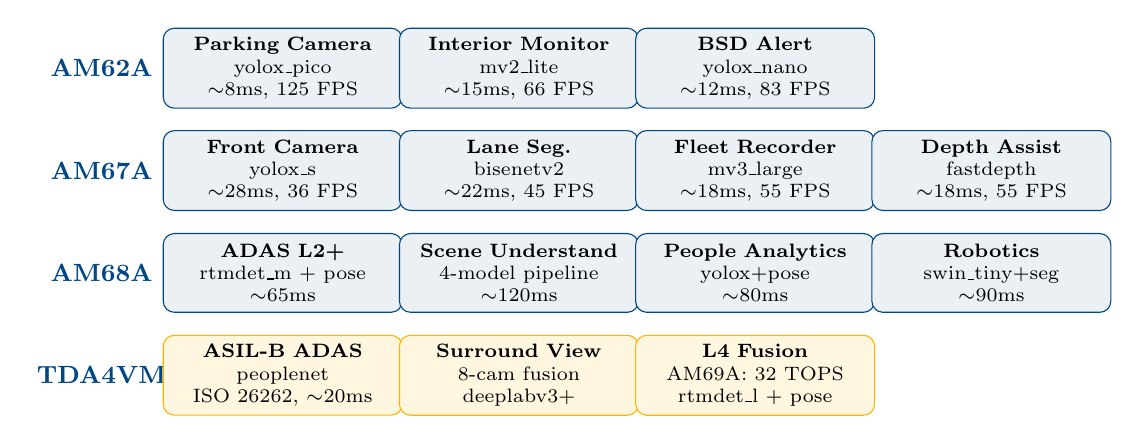
\begin{tikzpicture}[
  app/.style={draw=TIBlue,fill=TIBlue!8,rounded corners=4pt,
              minimum height=1.0cm,text width=2.8cm,align=center,font=\scriptsize},
  gold/.style={draw=TIGold,fill=TIGold!12,rounded corners=4pt,
               minimum height=1.0cm,text width=2.8cm,align=center,font=\scriptsize},
  soclbl/.style={font=\small\bfseries,text=TIBlue},
]
\node[soclbl] at (-0.8,4.2) {AM62A};
\node[app] at (1.5,4.2) {\textbf{Parking Camera}\\yolox\_pico\\$\sim$8ms, 125 FPS};
\node[app] at (4.5,4.2) {\textbf{Interior Monitor}\\mv2\_lite\\$\sim$15ms, 66 FPS};
\node[app] at (7.5,4.2) {\textbf{BSD Alert}\\yolox\_nano\\$\sim$12ms, 83 FPS};
\node[soclbl] at (-0.8,2.9) {AM67A};
\node[app] at (1.5,2.9) {\textbf{Front Camera}\\yolox\_s\\$\sim$28ms, 36 FPS};
\node[app] at (4.5,2.9) {\textbf{Lane Seg.}\\bisenetv2\\$\sim$22ms, 45 FPS};
\node[app] at (7.5,2.9) {\textbf{Fleet Recorder}\\mv3\_large\\$\sim$18ms, 55 FPS};
\node[app] at (10.5,2.9) {\textbf{Depth Assist}\\fastdepth\\$\sim$18ms, 55 FPS};
\node[soclbl] at (-0.8,1.6) {AM68A};
\node[app] at (1.5,1.6) {\textbf{ADAS L2+}\\rtmdet\_m + pose\\$\sim$65ms};
\node[app] at (4.5,1.6) {\textbf{Scene Understand}\\4-model pipeline\\$\sim$120ms};
\node[app] at (7.5,1.6) {\textbf{People Analytics}\\yolox+pose\\$\sim$80ms};
\node[app] at (10.5,1.6) {\textbf{Robotics}\\swin\_tiny+seg\\$\sim$90ms};
\node[soclbl] at (-0.8,0.3) {TDA4VM};
\node[gold] at (1.5,0.3) {\textbf{ASIL-B ADAS}\\peoplenet\\ISO 26262, $\sim$20ms};
\node[gold] at (4.5,0.3) {\textbf{Surround View}\\8-cam fusion\\deeplabv3+};
\node[gold] at (7.5,0.3) {\textbf{L4 Fusion}\\AM69A: 32 TOPS\\rtmdet\_l + pose};
\end{tikzpicture}
\end{frame}

\begin{frame}{ADAS NCAP Scenario: Multi-Model Pipeline on AM68A}
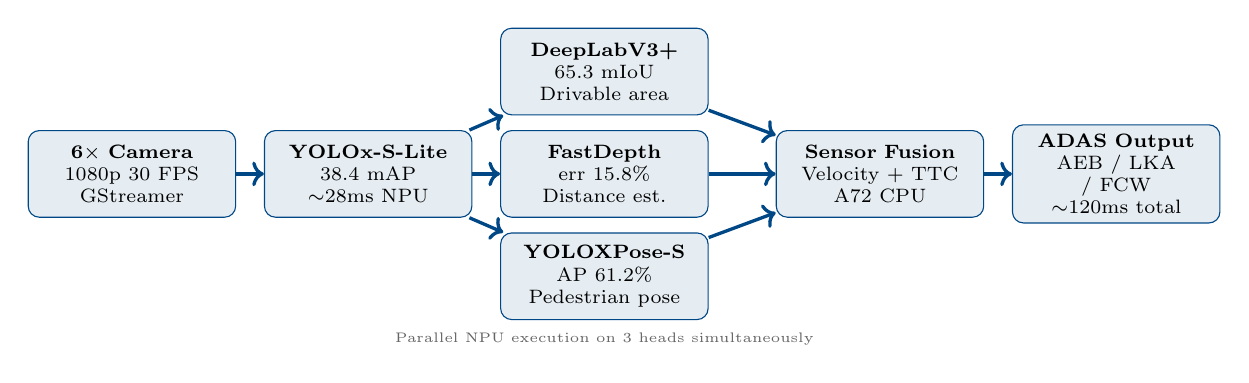
\begin{tikzpicture}[
  blk/.style={draw=TIBlue,fill=TIBlue!10,rounded corners=4pt,
              minimum height=1.1cm,text width=2.4cm,align=center,font=\scriptsize},
  arr/.style={->,line width=1.2pt,TIBlue},
]
\node[draw=TIGray,fill=LightGray,blk] (cam) at (0,1.5)
  {\textbf{6$\times$ Camera}\\1080p 30 FPS\\GStreamer};
\node[blk] (det) at (3,1.5)
  {\textbf{YOLOx-S-Lite}\\38.4 mAP\\$\sim$28ms NPU};
\node[blk] (seg) at (6,2.8)
  {\textbf{DeepLabV3+}\\65.3 mIoU\\Drivable area};
\node[blk] (dep) at (6,1.5)
  {\textbf{FastDepth}\\err 15.8\%\\Distance est.};
\node[blk] (pose) at (6,0.2)
  {\textbf{YOLOXPose-S}\\AP 61.2\%\\Pedestrian pose};
\node[draw=TIRed,fill=TIRed!10,blk] (fuse) at (9.5,1.5)
  {\textbf{Sensor Fusion}\\Velocity + TTC\\A72 CPU};
\node[draw=TIGold,fill=TIGold!15,blk] (adas) at (12.5,1.5)
  {\textbf{ADAS Output}\\AEB / LKA / FCW\\$\sim$120ms total};
\draw[arr] (cam) -- (det);
\draw[arr] (det) -- (seg);
\draw[arr] (det) -- (dep);
\draw[arr] (det) -- (pose);
\draw[arr] (seg) -- (fuse);
\draw[arr] (dep) -- (fuse);
\draw[arr] (pose) -- (fuse);
\draw[arr] (fuse) -- (adas);
\node[font=\tiny,text=TIGray] at (6.0,-0.6)
  {Parallel NPU execution on 3 heads simultaneously};
\end{tikzpicture}
\end{frame}

% ════════════════════════════════════════════════
\section{Development Ecosystem}
% ════════════════════════════════════════════════

\begin{frame}{TI EdgeAI Development Ecosystem}
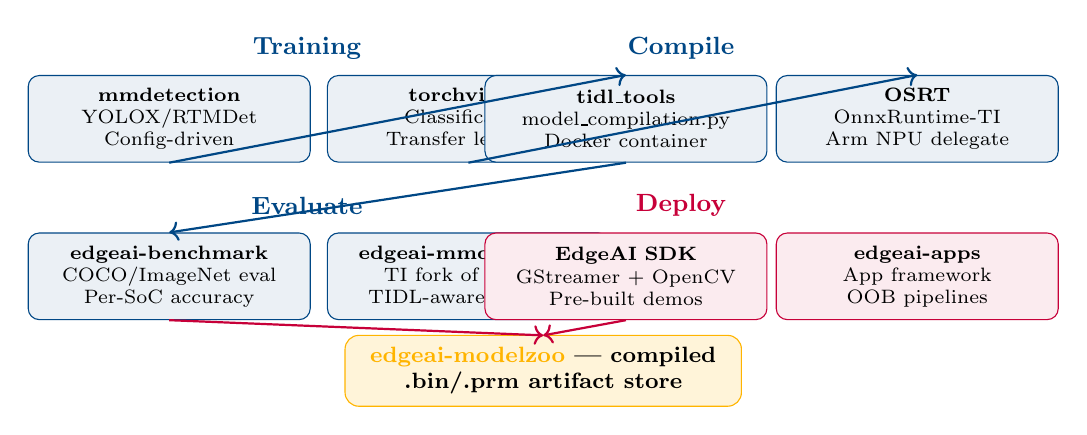
\begin{tikzpicture}[
  tool/.style={draw=TIBlue,fill=TIBlue!8,rounded corners=4pt,
               minimum width=3.5cm,minimum height=1.1cm,
               text width=3.3cm,align=center,font=\scriptsize,inner sep=4pt},
  rtool/.style={draw=TIRed,fill=TIRed!8,rounded corners=4pt,
                minimum width=3.5cm,minimum height=1.1cm,
                text width=3.3cm,align=center,font=\scriptsize,inner sep=4pt},
]
\node[font=\small\bfseries,text=TIBlue] at (1.75,5.2) {Training};
\node[tool] (mmdet) at (0,4.3)
  {\textbf{mmdetection}\\YOLOX/RTMDet\\Config-driven};
\node[tool] (torchv) at (3.8,4.3)
  {\textbf{torchvision}\\Classification\\Transfer learning};
\node[font=\small\bfseries,text=TIBlue] at (6.5,5.2) {Compile};
\node[tool] (tidlt) at (5.8,4.3)
  {\textbf{tidl\_tools}\\model\_compilation.py\\Docker container};
\node[tool] (osrt) at (9.5,4.3)
  {\textbf{OSRT}\\OnnxRuntime-TI\\Arm NPU delegate};
\node[font=\small\bfseries,text=TIBlue] at (1.75,3.2) {Evaluate};
\node[tool] (bench) at (0,2.3)
  {\textbf{edgeai-benchmark}\\COCO/ImageNet eval\\Per-SoC accuracy};
\node[tool] (edmm) at (3.8,2.3)
  {\textbf{edgeai-mmdetection}\\TI fork of mmdet\\TIDL-aware training};
\node[font=\small\bfseries,text=TIRed] at (6.5,3.2) {Deploy};
\node[rtool] (sdk) at (5.8,2.3)
  {\textbf{EdgeAI SDK}\\GStreamer + OpenCV\\Pre-built demos};
\node[rtool] (apps) at (9.5,2.3)
  {\textbf{edgeai-apps}\\App framework\\OOB pipelines};
\node[draw=TIGold,fill=TIGold!15,rounded corners=5pt,
      minimum width=5cm,minimum height=0.9cm,
      text width=4.8cm,align=center,font=\footnotesize\bfseries]
  at (4.75,1.1) {\textcolor{TIGold}{\textbf{edgeai-modelzoo}} --- compiled .bin/.prm artifact store};
\draw[->,TIBlue,line width=0.8pt] (mmdet.south) -- (tidlt.north);
\draw[->,TIBlue,line width=0.8pt] (torchv.south) -- (osrt.north);
\draw[->,TIBlue,line width=0.8pt] (tidlt.south) -- (bench.north);
\draw[->,TIRed,line width=0.8pt] (bench.south) -- (4.75,1.55);
\draw[->,TIRed,line width=0.8pt] (sdk.south) -- (4.75,1.55);
\end{tikzpicture}
\end{frame}

\begin{frame}{GStreamer Pipeline: Camera to NPU in 10 Lines}
\begin{columns}
\column{0.55\textwidth}
\small
\begin{block}{Typical GStreamer App}
\footnotesize
\begin{verbatim}
gst-launch-1.0 \
  v4l2src device=/dev/video0 ! \
  video/x-raw,width=1280,height=720 ! \
  tiovxdlpreproc model=yolox_s.bin \
                 out-pool-size=4 ! \
  tidlinferer model=yolox_s.bin \
              model-perf=yolox_s.prm ! \
  tiovxdlpostproc \
    model=yolox_s.bin \
    viz-threshold=0.5 ! \
  kmssink sync=false
\end{verbatim}
\end{block}
\column{0.42\textwidth}
\footnotesize
\begin{block}{Pipeline Stages}
\begin{itemize}
  \item \textbf{v4l2src}: camera capture
  \item \textbf{tiovxdlpreproc}: resize, normalize on NPU
  \item \textbf{tidlinferer}: TIDL .bin inference
  \item \textbf{tiovxdlpostproc}: decode bboxes, draw
  \item \textbf{kmssink}: display HDMI output
\end{itemize}
\end{block}
\begin{alertblock}{Zero extra Python code}
\footnotesize All TIDL NPU inference, pre/post-processing runs inside the GStreamer plugin --- no Python overhead on the hot path.
\end{alertblock}
\end{columns}
\end{frame}

\begin{frame}{MLOps Pipeline for TI EdgeAI}
\small
\begin{tabular}{llll}
\toprule
\textbf{Stage} & \textbf{Tool} & \textbf{Artifact} & \textbf{Gate}\\
\midrule
Experiment tracking & MLflow & run metrics, params & ---\\
Calibration \& compile & TIDL + Optuna HPO & .bin + .prm & Acc drop $<$2\%\\
Model registry & MLflow Registry & Staging $\to$ Production & mAP $>$ threshold\\
Orchestration & Prefect 2 flows & DAG with retries & Task-level SLAs\\
Drift detection & Evidently AI & Confidence + Acc drift & $>$5\% drift $\to$ alert\\
CI/CD & GitHub Actions & 6-job pipeline & All gates pass\\
Infrastructure & AWS CDK v2 & S3+ECR+ECS+CW & CloudWatch alarms\\
\bottomrule
\end{tabular}
\vspace{0.3cm}
\begin{block}{Optuna HPO for TIDL Compile}
\footnotesize Tunes: \texttt{num\_bits} (8 vs 16), \texttt{num\_calibration\_frames} (50--500), \texttt{max\_mem\_banks} (8--64), \texttt{deny\_list\_layers} (which layers stay FP32). Objective: maximize accuracy subject to latency $<$ target\_ms.
\end{block}
\end{frame}

% ════════════════════════════════════════════════
\section{Summary}
% ════════════════════════════════════════════════

\begin{frame}{Summary: TI EdgeAI at a Glance}
\begin{columns}
\column{0.52\textwidth}
\small
\begin{tabular}{lcc}
\toprule
\textbf{Dimension} & \textbf{Score} & \textbf{Notes}\\
\midrule
Model variety      & $\bigstar\bigstar\bigstar\bigstar\bigstar$ & 34 models, 5 tasks\\
Classification acc.& $\bigstar\bigstar\bigstar\bigstar\bigstar$ & 81.2\% swin\_tiny\\
Detection acc.     & $\bigstar\bigstar\bigstar\bigstar\bigstar$ & 60\% rtmdet\_l\\
Power efficiency   & $\bigstar\bigstar\bigstar$                 & 3--30W range\\
Quantization ease  & $\bigstar\bigstar\bigstar\bigstar$         & PTQ, 50 frames\\
NPU coverage       & $\bigstar\bigstar\bigstar\bigstar\bigstar$ & $>$95\% on NPU\\
Dev.\ ecosystem    & $\bigstar\bigstar\bigstar\bigstar\bigstar$ & SDK + GStreamer\\
Safety readiness   & $\bigstar\bigstar\bigstar\bigstar$         & TDA4VM ASIL-B\\
\bottomrule
\end{tabular}
\vspace{0.2cm}
\footnotesize
\begin{tabular}{lcc}
\toprule
\textbf{SoC} & \textbf{TOPS} & \textbf{Recommended task}\\
\midrule
AM62A  & 1  & Parking, BSD, driver monitor\\
AM67A  & 4  & Front cam ADAS, fleet, depth\\
AM68A  & 8  & L2+ ADAS, robotics, people\\
AM69A  & 32 & L4, multi-sensor, 8 cameras\\
TDA4VM & 8  & Automotive OEM, ASIL-B\\
\bottomrule
\end{tabular}
\column{0.45\textwidth}
\begin{block}{Key Differentiators}
\begin{itemize}
  \item \textbf{34 vision models} --- largest vision zoo
  \item \textbf{\_lite model family} co-designed for TIDL INT8 PTQ
  \item \textbf{$>$95\% FLOPs on NPU} for all CNN models
  \item \textbf{ASIL-B capable} via TDA4VM + peoplenet
  \item \textbf{GStreamer SDK} for camera-to-output in $<$10 lines
  \item \textbf{Multi-model pipelines}: 4-stage ADAS at 8 FPS
\end{itemize}
\end{block}
\begin{alertblock}{Best Fit When\ldots}
\footnotesize Automotive or industrial applications need vision intelligence at 30+ FPS with the highest detection accuracy, a complete deployment SDK, and optional ASIL-B safety path.
\end{alertblock}
\end{columns}
\end{frame}

\end{document}
